% GNUPLOT: LaTeX picture with Postscript
\begingroup
  \makeatletter
  \providecommand\color[2][]{%
    \GenericError{(gnuplot) \space\space\space\@spaces}{%
      Package color not loaded in conjunction with
      terminal option `colourtext'%
    }{See the gnuplot documentation for explanation.%
    }{Either use 'blacktext' in gnuplot or load the package
      color.sty in LaTeX.}%
    \renewcommand\color[2][]{}%
  }%
  \providecommand\includegraphics[2][]{%
    \GenericError{(gnuplot) \space\space\space\@spaces}{%
      Package graphicx or graphics not loaded%
    }{See the gnuplot documentation for explanation.%
    }{The gnuplot epslatex terminal needs graphicx.sty or graphics.sty.}%
    \renewcommand\includegraphics[2][]{}%
  }%
  \providecommand\rotatebox[2]{#2}%
  \@ifundefined{ifGPcolor}{%
    \newif\ifGPcolor
    \GPcolorfalse
  }{}%
  \@ifundefined{ifGPblacktext}{%
    \newif\ifGPblacktext
    \GPblacktexttrue
  }{}%
  % define a \g@addto@macro without @ in the name:
  \let\gplgaddtomacro\g@addto@macro
  % define empty templates for all commands taking text:
  \gdef\gplbacktext{}%
  \gdef\gplfronttext{}%
  \makeatother
  \ifGPblacktext
    % no textcolor at all
    \def\colorrgb#1{}%
    \def\colorgray#1{}%
  \else
    % gray or color?
    \ifGPcolor
      \def\colorrgb#1{\color[rgb]{#1}}%
      \def\colorgray#1{\color[gray]{#1}}%
      \expandafter\def\csname LTw\endcsname{\color{white}}%
      \expandafter\def\csname LTb\endcsname{\color{black}}%
      \expandafter\def\csname LTa\endcsname{\color{black}}%
      \expandafter\def\csname LT0\endcsname{\color[rgb]{1,0,0}}%
      \expandafter\def\csname LT1\endcsname{\color[rgb]{0,1,0}}%
      \expandafter\def\csname LT2\endcsname{\color[rgb]{0,0,1}}%
      \expandafter\def\csname LT3\endcsname{\color[rgb]{1,0,1}}%
      \expandafter\def\csname LT4\endcsname{\color[rgb]{0,1,1}}%
      \expandafter\def\csname LT5\endcsname{\color[rgb]{1,1,0}}%
      \expandafter\def\csname LT6\endcsname{\color[rgb]{0,0,0}}%
      \expandafter\def\csname LT7\endcsname{\color[rgb]{1,0.3,0}}%
      \expandafter\def\csname LT8\endcsname{\color[rgb]{0.5,0.5,0.5}}%
    \else
      % gray
      \def\colorrgb#1{\color{black}}%
      \def\colorgray#1{\color[gray]{#1}}%
      \expandafter\def\csname LTw\endcsname{\color{white}}%
      \expandafter\def\csname LTb\endcsname{\color{black}}%
      \expandafter\def\csname LTa\endcsname{\color{black}}%
      \expandafter\def\csname LT0\endcsname{\color{black}}%
      \expandafter\def\csname LT1\endcsname{\color{black}}%
      \expandafter\def\csname LT2\endcsname{\color{black}}%
      \expandafter\def\csname LT3\endcsname{\color{black}}%
      \expandafter\def\csname LT4\endcsname{\color{black}}%
      \expandafter\def\csname LT5\endcsname{\color{black}}%
      \expandafter\def\csname LT6\endcsname{\color{black}}%
      \expandafter\def\csname LT7\endcsname{\color{black}}%
      \expandafter\def\csname LT8\endcsname{\color{black}}%
    \fi
  \fi
  \setlength{\unitlength}{0.0500bp}%
  \begin{picture}(11520.00,8640.00)%
    \gplgaddtomacro\gplbacktext{%
      \colorrgb{0.00,0.00,0.00}%
      \put(1320,800){\makebox(0,0)[r]{\strut{}$0$}}%
      \colorrgb{0.00,0.00,0.00}%
      \put(1320,1536){\makebox(0,0)[r]{\strut{}$0.05$}}%
      \colorrgb{0.00,0.00,0.00}%
      \put(1320,2272){\makebox(0,0)[r]{\strut{}$0.1$}}%
      \colorrgb{0.00,0.00,0.00}%
      \put(1320,3008){\makebox(0,0)[r]{\strut{}$0.15$}}%
      \colorrgb{0.00,0.00,0.00}%
      \put(1320,3744){\makebox(0,0)[r]{\strut{}$0.2$}}%
      \colorrgb{0.00,0.00,0.00}%
      \put(1320,4480){\makebox(0,0)[r]{\strut{}$0.25$}}%
      \colorrgb{0.00,0.00,0.00}%
      \put(1320,5215){\makebox(0,0)[r]{\strut{}$0.3$}}%
      \colorrgb{0.00,0.00,0.00}%
      \put(1320,5951){\makebox(0,0)[r]{\strut{}$0.35$}}%
      \colorrgb{0.00,0.00,0.00}%
      \put(1320,6687){\makebox(0,0)[r]{\strut{}$0.4$}}%
      \colorrgb{0.00,0.00,0.00}%
      \put(1320,7423){\makebox(0,0)[r]{\strut{}$0.45$}}%
      \colorrgb{0.00,0.00,0.00}%
      \put(1320,8159){\makebox(0,0)[r]{\strut{}$0.5$}}%
      \colorrgb{0.00,0.00,0.00}%
      \put(1560,400){\makebox(0,0){\strut{}$0$}}%
      \colorrgb{0.00,0.00,0.00}%
      \put(2792,400){\makebox(0,0){\strut{}$2 \cdot 10^{4}$}}%
      \colorrgb{0.00,0.00,0.00}%
      \put(4024,400){\makebox(0,0){\strut{}$4 \cdot 10^{4}$}}%
      \colorrgb{0.00,0.00,0.00}%
      \put(5256,400){\makebox(0,0){\strut{}$6 \cdot 10^{4}$}}%
      \colorrgb{0.00,0.00,0.00}%
      \put(6487,400){\makebox(0,0){\strut{}$8 \cdot 10^{4}$}}%
      \colorrgb{0.00,0.00,0.00}%
      \put(7719,400){\makebox(0,0){\strut{}$10 \cdot 10^{4}$}}%
      \colorrgb{0.00,0.00,0.00}%
      \put(8951,400){\makebox(0,0){\strut{}$12 \cdot 10^{4}$}}%
      \colorrgb{0.00,0.00,0.00}%
      \put(10183,400){\makebox(0,0){\strut{}$14 \cdot 10^{4}$}}%
    }%
    \gplgaddtomacro\gplfronttext{%
      \csname LTb\endcsname%
      \put(9056,7896){\makebox(0,0)[r]{\strut{}$\theta_{exp}= \:\: 4$}}%
      \csname LTb\endcsname%
      \put(9056,7496){\makebox(0,0)[r]{\strut{}$\theta_{exp}=20$}}%
      \csname LTb\endcsname%
      \put(9056,7096){\makebox(0,0)[r]{\strut{}$\theta_{exp}=40$}}%
    }%
    \gplbacktext
    \put(0,0){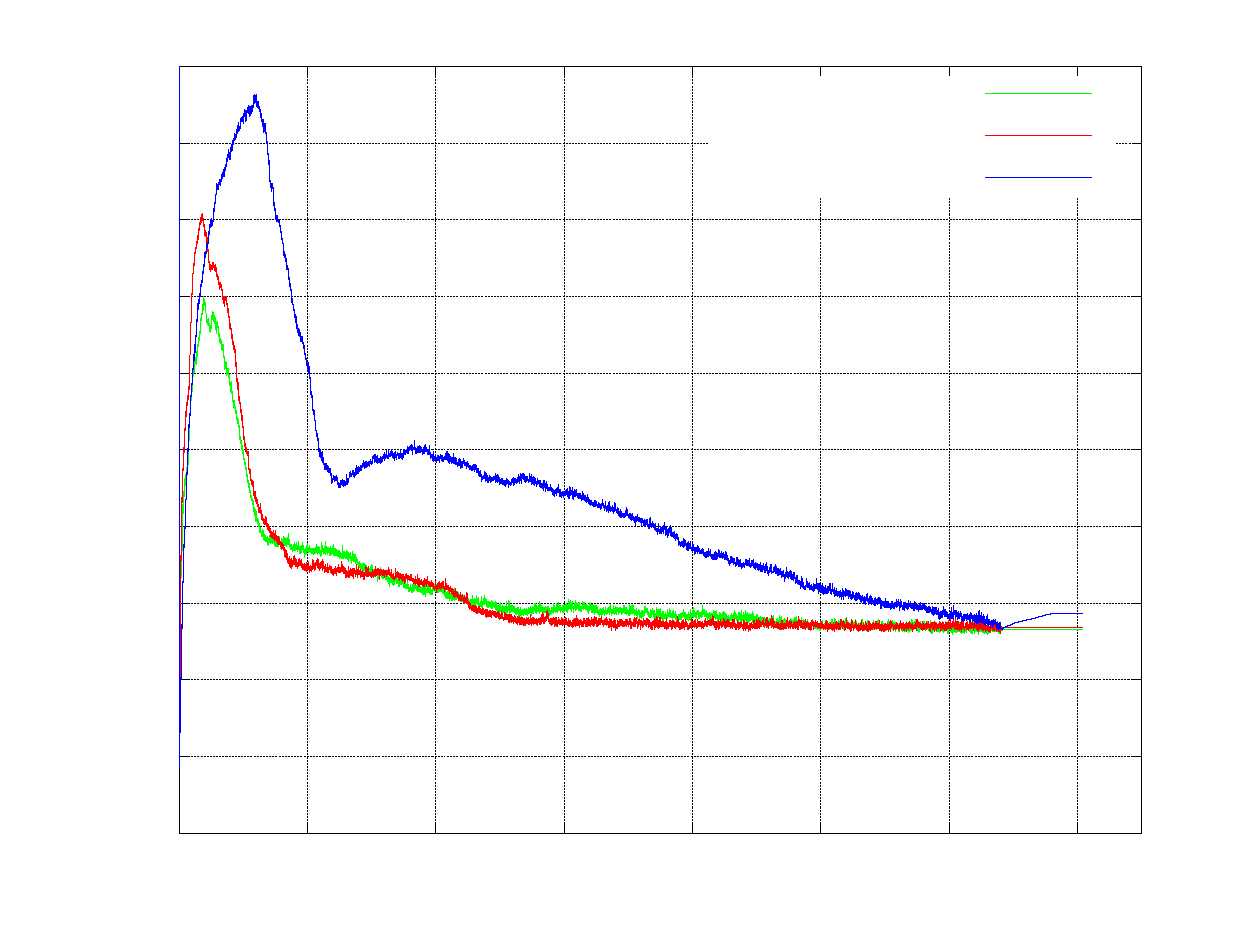
\includegraphics{./images/mlPosition7ThetaGA.eps}}%
    \gplfronttext
  \end{picture}%
\endgroup
